\section{Dataset Description}

The dataset for this project was obtained from a Kaggle repository titled \textit{Dangerous Heartbeat Dataset (DHD)} \cite{Dangerous-Heartbeat-Dataset-DHD}, 
which in turn sources its data from the PASCAL Classifying Heart Sounds Challenge 2011 (CHSC2011) \cite{pascal-chsc-2011}. 
This dataset comprises audio recordings of heartbeats, categorized into different types of heart sounds.
Specifically, the dataset consists of 5 types of recordings: Normal Heart Sounds, Murmur Sounds, Extra Heart Sounds, Extrasystole Sounds, and Artifacts.
Data has been gathered from the general public via the iStethoscope Pro iPhone app and from a clinic trial in hospitals using the digital stethoscope DigiScope.

\subsection{Data Distribution}
Figure \ref{fig:DataExp_num_durations}, show the presence of highly imbalanced classes in the dataset.
This poses a challenge for the classification task as the model may not have enough samples to learn from,
especially for the 'Extrastole' and 'Extrahls' classes. This problem is tackled trying to augment the data available,
both by segmenting the audio files and by using data augmentation techniques. Furthermore, 
we test the effectiveness of oversampling and undersampling techniques on the model performance.
The data is split intro training and testing sets, with a 80\% - 20\% ratio, respectively. The validation set
is omitted, due to the low number of samples available.

\begin{figure}[H]
    \centering
    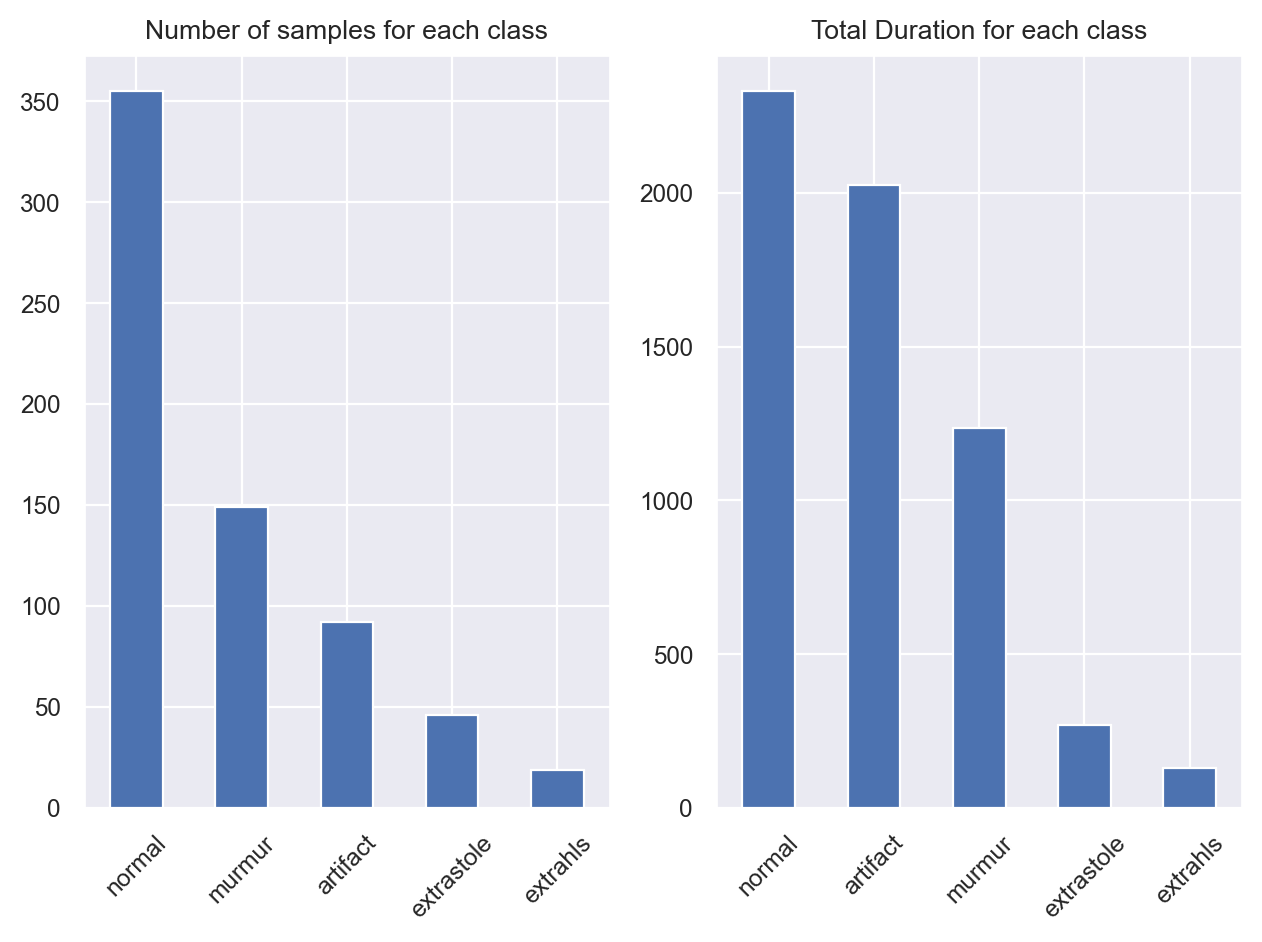
\includegraphics[width=1\columnwidth]{./images/DataExp_num_durations.png}
    \caption{Number of samples per duration.}
    \label{fig:DataExp_num_durations}
\end{figure}



\subsection{Data Preprocessing}
Here is a list of the preprocessing operations performed on the dataset:

\vspace{0.3cm}\noindent
\textbf{Noise Reduction:} the audio data was already provided in a clipped format 
to minimize noise and irrelevant information.

\vspace{0.3cm}\noindent
\textbf{Removal of Corrupted Files:} corrupted files were identified and removed 
from the dataset to ensure data quality.

\vspace{0.3cm}\noindent
\textbf{Resampling:} all audio files were resampled to a common frequency of 4000 Hz, 
which was identified as the optimal sampling rate (see Section \ref{sec:sr_extraction_interval}).

\vspace{0.3cm}\noindent
\textbf{Segmentation:} the audio data was segmented into 1-second intervals, 
identified as the optimal extraction interval (see Section \ref{sec:sr_extraction_interval}).

\vspace{0.3cm}\noindent
\textbf{Outlier Detection and Removal:} we investigated the average duration of 
each class and found that the 'artifact' class had a significantly larger average 
duration. This was due to a few lengthy audio 
recordings (see Figure \ref{fig:DataExp_outliers_Artifacts}). These recordings were 
considered as outliers and removed from the dataset, as a large number of samples from 
the same audio might not be as informative.

\begin{figure}[H]
	\centering
	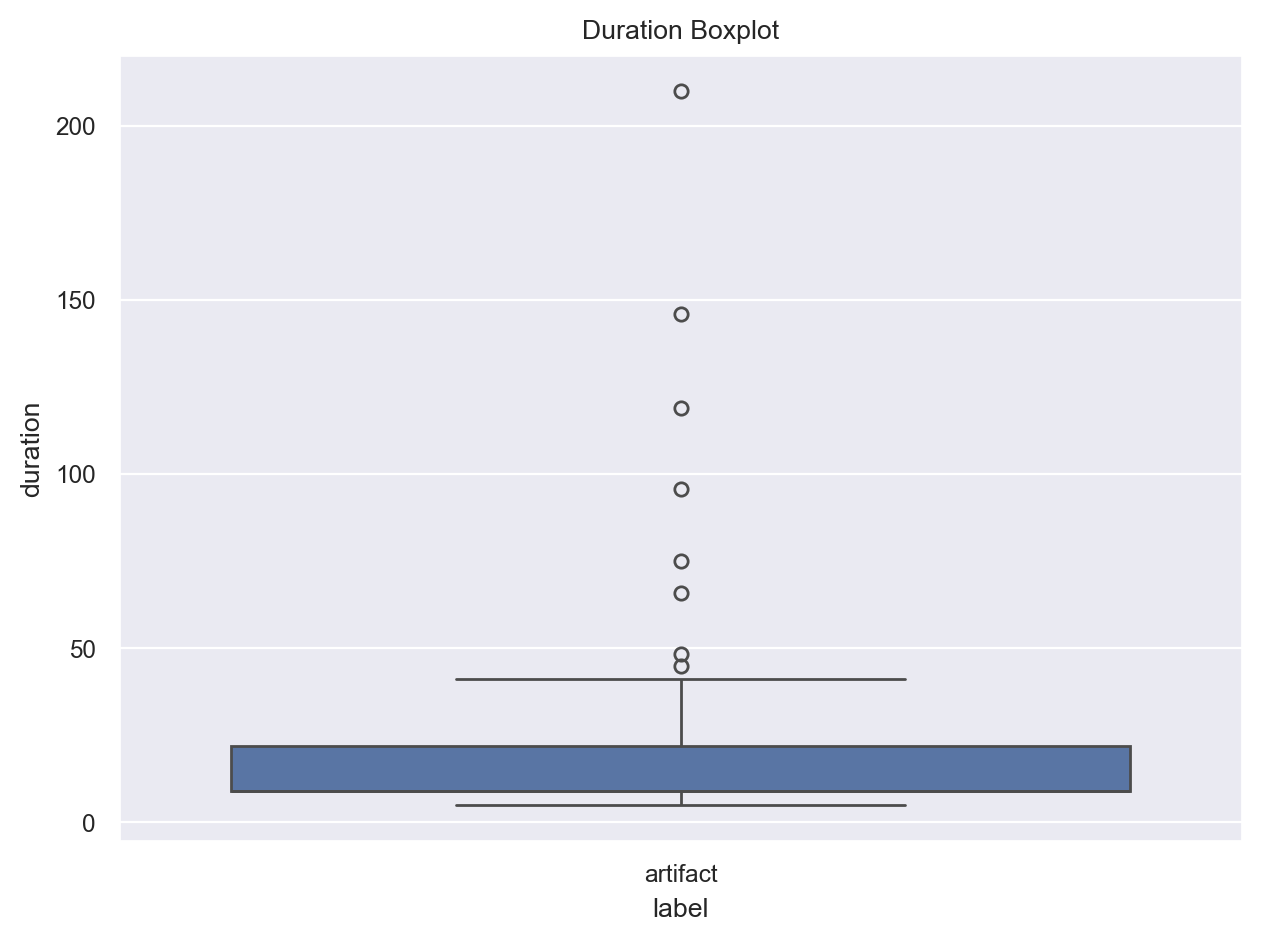
\includegraphics[width=1\columnwidth]{./images/DataExp_outliers_artifact.png}
	\caption{Outliers in the Artifacts class.}
	\label{fig:DataExp_outliers_Artifacts}
 \end{figure}